\chapter{Experimental Work}
\label{ch:experimental_work}
This chapter describes the experimental work done as part of the project. Since it is a rather incremental process, the goal, procedure and relevant results are described individually in each section.

\section{Implementation of a Runtime Support System for State Machines in Lua}
\label{sec:impl_runtime_support}
The first step towards working with state machine -based applications, is building a runtime system for a collection of generalized state machines. For the experimental purposes of this project, a runtime system with only the most basic functionality is needed. The components required for this are:

\begin{itemize}
	\item An \emph{event} data structure for handling messages to and between state machines
	\item A \emph{timer} object for keeping track of timed events
	\item A prototype/\gls{api} for state machines
	\item A \emph{scheduler} to keep track of active state machines, events and timers, and assigning events and timers to their respective state machines at the appropriate time.
\end{itemize}

It turns out to be quite simple to implement this system in Lua. The source code is included in Appx.~\ref{code:rts}, and each component is explained in the sections below.

\subsection{Event Data Structure}
\label{sec:impl_event}
Even though Lua is not natively object-oriented, an event object is still easily implemented by use of the \emph{\_\_index} metamethod~\cite[13.4.1]{book:programming_in_lua_first}. We simply create a prototype for the event object with the desired fields (ID of state machine, event type and additional data) and methods (constructor, setters and getters). Inheritance is then enabled by creating an empty table/object, and setting its \emph{\_\_index} to reference the parent object's fields. Lua doesn't support encapsulation by conventional means~\cite[16.4]{book:programming_in_lua_first}, but rather by creating \emph{closures}. Encapsulated fields may then only be accessed by functions declared in the same local scope, as seen in the constructor method for event (\emph{Event:new}, Code snip.~\ref{code:event}). This is useful also in a state machine context to avoid inadvertent or even malicious tampering with event data or state of state machines. Combined, these approaches make the event data structure simple, safe and easy to use.

\subsection{Timer Object}
\label{sec:impl_timer}
The timer object (Code snip.~\ref{code:timer}) is created similarly to the event object described in Sect.~\ref{sec:impl_event} with respect to inheritance and encapsulation. Additionally, we need some way to keep track of time. As discussed in Sect.~\ref{sec:lua_and_state_machines}, Lua does not natively offer preemptive multitasking, so running an active timer on a separate thread is pretty much out of the question. However, for a simple runtime system, we may delegate the responsibility of measuring time to the scheduler component, and simply create a \emph{timestamp} for the desired activation time. This may decrease the timing accuracy of activation, but on the other hand also decreases overhead and complexity of the runtime system. In many cases it is not necessary or even desirable to preempt a running transition, but sufficient to wait until the transition has finished before scheduling the event following the timeout. This is however something that should be addressed when designing a more complete runtime system, and something that may prove challenging, as discussed in Sect.~\ref{sec:lua_and_state_machines}.

The granularity of the timestamp is another issue that must be addressed, and is also discussed in Sect.~\ref{sec:lua_and_state_machines}. As a starting point, I chose to use \emph{os.time()}, even though it only offers \emph{second}-granularity. This is OK for the preliminary examples, and further addressed in Sect.~\ref{sec:running_on_micro}.

\subsection{State Machine Prototype/API}
\label{sec:impl_stm}
The third component we need is a prototype for implementation of a given state machine. This prototype serves as a kind of API, defining some common values and methods for all state machines. The state machine prototype (Code snip.~\ref{code:stm}), inspired by an exercise given in the course TTM4160 at NTNU, contains some predefined values to be returned to the scheduler after a transition, encapsulated data fields for state and ID, as well as a \emph{fire} function meant to be overridden in an implementation. When overridden, this function should implement all possible transitions for the state machine inside an eternal \emph{while}-loop such that only one transition is executed each pass.

Additionally, the required presence of a \emph{run} field holding a coroutine is indicated. The coroutine scheme is probably what makes the Lua implementation most unique. The coroutine references the \emph{fire} function, causing this function to be \emph{resumed} when the coroutine is resumed. This coroutine scheme fits perfectly into our runtime system as a way of structuring the program. Each state machine has its own coroutine with a separate thread, maintaining its state as well as other data, while the scheduler (see Sect. \ref{sec:impl_sched}) runs the main thread, handing execution control over to state machines according to events and timeouts. As a result of this, a state machine transition is never interrupted by a scheduler, meaning we have to trust all state machines to eventually hand execution control back to the scheduler. On the other hand, we don't have to worry about making state machines or transitions ``thread safe''.

\subsection{Scheduler}
\label{sec:impl_sched}
The scheduler (Code snip.~\ref{code:scheduler}) is the last component we need for our runtime system, and this is where the flexible properties of Lua tables really come into play. The scheduler needs to provide a set of functions enabling the following:

\begin{itemize}
	\item Adding and removing state machines
	\item Adding and keeping track of new events
	\item Adding, removing (stopping) and keeping track of timers
	\item Scheduling of events and timers (timeouts) to their respective state machines in an appropriate order
\end{itemize}

Adding and removing state machines is enabled by keeping a table with references to active state machine objects, indexed by their ID. Similar schemes are implemented for events and timers. Lua tables natively allow indexing by arbitrary values, as well as inserting at the end or removing from the front, effectively emulating the semantics of a hashmap or a queue without the need for any extra tweaking or import of libraries. The list of timers is kept sorted to make checking for timeouts quicker, but at the cost of extra work on insertion (with busy waiting, checking timers is generally done a lot more often than adding new timers).

Finally, we have a continuously running \emph{run} function that handles the actual scheduling. The scheduling scheme is kept simple: timeouts have priority over events. For each pass, the function first checks if any timers have expired, and if not, moves on to check if there are any events waiting. If a timeout or event is found, execution control is handed to the state machine it belongs to with a \emph{coroutine.resume} call. The scheduler thread then waits until the following transition is completed, and execution control is returned from the state machine through the \emph{coroutine.yield} call, before doing another pass.

\subsection{Missing Features and Possible Issues}
While the most basic functionality is easy to implement, the runtime system outlined in the previous sections far from complete. It is probably sufficient for very basic state machine applications that don't have, for example, strict timing requirements or external event sources. These issues should be considered when designing a more complete system.

\paragraph{Multitasking} The main issue to consider here is probably multitasking. For a simple scheme where only the internal state machines are generating events, non-preemptive multitasking is a great solution. However, in many cases sources of events will be external to the system like in the case of an Ethernet socket. With only one thread executing at a time, receiving external events asynchronously is difficult. Most likely we need another process running in parallel, listening for events and adding them to the queue as they arrive, which in most cases means preemptive multitasking, however shared memory/pipes may also be an option. Additionally, an ill-defined state machine may get stuck in a transition, never returning control to the scheduler. In this case, it could have been wise to have a \emph{watchdog timer} running in parallel, ready to hand control back to the scheduler if the transition takes too long. Standard Lua does not offer any way of doing this though, so our options are to use external libraries or write our own multitasking module. Some Lua libraries implementing preemptive multitasking exist, but I have left these out for now, as they rely on threads in the underlying operating system, which will not be available when we move on to the microcontroller in Sect.~\ref{sec:running_on_micro}.

\paragraph{Timing Accuracy} Another point we need to consider, is timeout accuracy. Since timers are not allowed to preempt, execution may be delayed for an unknown amount of time. Again, this is probably ok if you don't require very strict timing accuracy, but this may not always be the case. Unfortunately, better guarantees for timing accuracy is hard to achieve without preemptive multitasking.

\paragraph{Saving Events}

\paragraph{Busy Waiting}

\section{Implementation of State Machines in Lua}
\label{sec:impl_state_machines}
When we have a working runtime system, the next step is to create state machines implementing the application we want to create. The following sections provide some examples of simple state machine applications, based on the prototype described in Sect.~\ref{sec:impl_stm}.

\subsection{The Traffic Light Controller State Machine}
\label{sec:impl_traffic_light}
Like the state machine prototype, the Traffic Light Controller is inspired by an exercise given in the TTM4160 course. In this application, we simulate a controller for a pedestrian traffic light. When a pedestrian pushes the button, the light for cars is set to yellow, and a timer is started. Following the resulting timeout, lights are set to new colors and new timers are started accordingly, until the whole sequence is complete, and the controller waits for a new button press. Its \gls{uml} specification is shown in Fig.~\ref{fig:traffic_light_uml}, and the resulting Lua code in Code snip.~\ref{code:traffic_light}\footnote{Also available on GitHub: \url{https://github.com/Desarc/state_machine_rts/tree/master/trafficlight}}.

The Lua code is fairly straightforward: we load required modules and define some constants specific to this state machine, like states, timer delays, and event types. The next step is to create a simple constructor, assigning a given ID to the new Traffic Light Controller instance, setting the initial state, and keeping a reference to the scheduler. The final part is the \emph{fire} function looping over all the possible transitions. This is implemented in an action-oriented way, making the code clearly structured and very readable. Every transition fork ends with a call to \emph{coroutine.yield}, handling execution control back to the scheduler. It is really important to end every possible fork with a yield as done with the numerous \emph{else} statements, or we risk the state machine getting stuck in the loop in case of an unexpected event.

Testing the application is equally straightforward: we create a \emph{main} program (Code snip.~\ref{code:main}) with an instance of the scheduler and the Traffic Light controller, and register the state machine with the scheduler. We also create a ``fake'' button press event, and add it to the scheduler's event queue. Finally, we start the runtime system by calling the scheduler's \emph{run} function, and observe the following behavior.

A test run of this application provided the output displayed in Fig.~\ref{fig:traffic_light_output}, with the appropriate timer delays between each line. This is in line with what we would expect from the \gls{uml} specification in Fig.~\ref{fig:traffic_light_uml}.

\begin{figure}[htp]
	\centering
	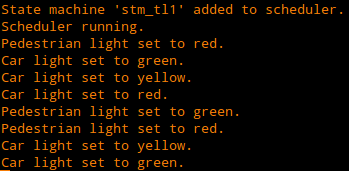
\includegraphics[scale=0.70]{traffic_light_output}
	\caption[Output of Traffic Light Controller test run]{Console output resulting from the test run of the Traffic Light Controller state machine application.}
	\label{fig:traffic_light_output}
\end{figure}

\subsection{Two Communicating Applications}
\label{sec:client_server_app}
Our next step is to test the runtime system with more than a single state machine, so the scheduler has to do some actual scheduling. To achieve this, I designed some simple state machines working together to form a client and a server. To communicate between the client and the server, I designed state machines using TCP sockets from the LuaSocket library\footnote{\url{http://w3.impa.br/~diego/software/luasocket/}}. The client application consists of one state machine for periodically generating requests (Fig.~\ref{fig:stm_event_gen}), one for displaying replies from the server (Fig.~\ref{fig:stm_print_message}) and one for sending and receiving messages over TCP (Fig.~\ref{fig:stm_client_conn}). The server application consists of one state machine for handling requests (Fig.~\ref{fig:stm_request_handler}) and one for sending and receiving messages over TCP (Fig.~\ref{fig:stm_server_conn})
The Lua implementation for the request generating state machine is displayed in Code snip.~\ref{code:event_gen}, and the remaining implementations are publicly available on GitHub\footnote{\url{https://github.com/Desarc/state_machine_rts/tree/master/client-server}}.

Comparing the implementation of the request generator to the implementation of the Traffic Light Controller in Sect.~\ref{sec:impl_traffic_light}, we see that a lot of the code may be reused. We basically only need to change state and event definitions, implement any operations performed in transitions, and finally change the action-oriented list of transitions to reflect those of the current state machine. It requires only minimal work, and is not particularly error-prone because the code is simple and readable. This also applies to the other state machines implemented for this application, and implies that creating more complex applications, given the state machine template and a working runtime system, should be rather trivial.

Running the two applications also produced the expected results: the client application periodically sends requests, these are handled by the server application, and the client application finally receives a response. The output produced is displayed in Fig.~\ref{fig:client_server_output}.

%\begin{figure}[htp]
%	\centering
%	\begin{subfigure}[b]{.4\textwidth}
%		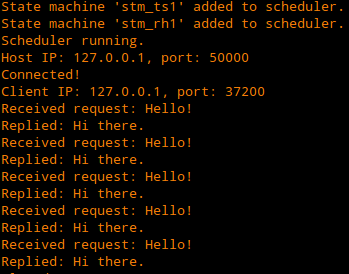
\includegraphics[scale=0.45]{server_output}
%		\caption{Server output}
%	\end{subfigure}
%	\quad
%	\begin{subfigure}[b]{.4\textwidth}
%		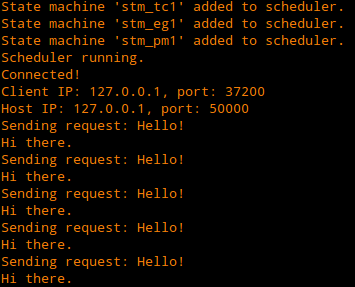
\includegraphics[scale=0.45]{client_output}
%		\caption{Client output}
%	\end{subfigure}
%	\caption{Console output from running the client and server applications.}
%	\label{fig:client_server_output}
%\end{figure}

\FloatBarrier
\subsection{Comparison to Generated State Machines}



\section{Running the State Machine Applications in an Embedded Environment}
\label{sec:running_on_micro}
Now that we have a working runtime system with a few example state machine -based applications, the next step is to see how this system performs in an embedded environment. In Sect.~\ref{sec:lua_in_embedded}, I looked into some previous efforts towards running the Lua interpreter in an embedded environment. Since porting Lua to an embedded environment is beyond the scope of this project, I chose to use \emph{eLua} with the supported Stellaris LM3S9D92 microcontroller as the platform for these experiments.

\subsection{The LM3S9D92 Microcontroller}
\label{sec:microcontroller}
The Stellaris LM3S9D92 is a microcontroller produced by Texas Instruments\footnote{\url{http://www.ti.com/product/lm3s9d92}}. It is considered outdated and \emph{``not recommended for new designs''}, but since the purpose of these experiments is to look into how our software performs in a resource-constrained environment, this is not a problem. The microcontroller was considered a \emph{``high performance microcontroller with large memory''}~\cite{website:stellaris_micro} when it was released, and has the following primary specifications:

\begin{itemize}
	\item 32-bit ARM Cortex-M3 processor
	\item 96KB SDRAM
	\item 512KB flash memory
\end{itemize}

Additionally, the evaluation kit used supports the following I/O peripherals:

\begin{itemize}
	\item Ethernet 10/100 port with two LED indicators
	\item User pushbutton and LED
	\item USB 2.0 Full-Speed OTG port
	\item Oversized board pads for GPIO access
\end{itemize}

Ethernet and TCP/IP is also supported by eLua for this platform, which should simplify the use of this feature in our state machines. Drivers interfacing with eLua for other peripherals do not seem to be present, but given eLua's open source, it should be possible to add these if needed.

\subsection{Running eLua on the Evaluation Kit Board}
\label{sec:running_elua}
In order to illustrate how quickly I was able to get the Lua interpreter up and running on the LM3S9D92, I have included a short description of the process in this section.

The first step was to get the interface to the evaluation kit board up and running. The board has an FTDI chip\footnote{\url{http://www.ftdichip.com/FTProducts.htm}} converting between USB and UART interfaces, so in order to communicate with the board we only need to connect it via USB. Texas Instruments also provide convenient desktop tools for connecting and flashing programs to the board, provided you are running on Windows. I simply had to install all the proper tools and drivers from the included CD, and turn the board on.

The next step was to get eLua running on the microcontroller. Using the flashing tool provided with the kit, I simply downloaded the appropriate binary image from the eLua website and copied it over.

The only challenge in this process was to find a suitable terminal emulator for Windows. The eLua wiki offered a few alternatives\footnote{\url{http://wiki.eluaproject.net/Terminal\%20Emulators\%20for\%20eLua}}, but many were outdated or didn't work properly. After trying out a few, I managed to connect using TeraTerm, and was able to run Lua scripts live through the eLua interpreter. Given the relative ease of this process, running Lua-based state machine applications seemed to be a very feasible option.

\subsection{Running the Initial State Machine Applications}
\label{sec:running_initial}
With Lua up and running on the evaluation kit board, the next step was to see if the runtime system with different state machine applications would run on it. In order to work on the embedded platform, some minor changes had to be done to the runtime system, particularly those that referenced \gls{os} functions. I had to replace the \emph{os.time()} function with the eLua \emph{tmr.read(tmr.SYS\_TIMER)} in the timer and scheduler objects. Also, because the eLua timers measure time in microseconds, I initially had to change all defined time constants. However, to make the difference between desktop and embedded versions of the runtime system a little smoother, I introduced a \emph{Timer.BASE} value representing the number of milliseconds in the timer object's base value for time measurement. This way we don't have to change timer constants in implemented state machines when changing from running in a desktop environment to running in an embedded environment.

\subsubsection{The Traffic Light Controller Application}


\subsubsection{The Client - Server Application}


\subsubsection{Considerations}




\section{Measurements of RTS performance Overhead}
\label{sec:overhead_measure}

\begin{listing}[h]
\begin{luacode}
local task_size = 10
local task_repeats = 1

local function busy_work()
	for i=1,task_size do
		q = i*i
	end
end

local start_time = tmr.read(tmr.SYS_TIMER)

for j=1,task_repeats do
	busy_work()
end

local delta = tmr.read(tmr.SYS_TIMER) - start_time
print("Delta: "..tostring(delta))
\end{luacode}
	\caption{Lua code used for overhead testing}
	\label{code:overhead}
\end{listing}

\section{Measurements of Application Performance}
\label{sec:performance_measure}

